\documentclass[conference]{IEEEtran}

%% Custom TeX

\usepackage{srcltx}
\usepackage{url}
%\usepackage{fullpage}
%\usepackage{fancyhdr}
\let\proof\relax
\let\endproof\relax
\usepackage{latexsym,amsthm,amsmath,amssymb,stmaryrd}

%\usepackage{charter}
%\usepackage{euler}
\renewcommand{\bfdefault}{b}

\usepackage{xspace}
\usepackage{enumerate}
%\usepackage[pdftex,hyperref,svgnames]{xcolor}
\usepackage{graphics}
%\usepackage{pstricks}
%\usepackage{color}
%\usepackage{comment}
\usepackage{listings}
\usepackage{supertabular}
\usepackage{stackrel}
\usepackage{marvosym}
\usepackage{pgf,tikz}
\usepackage{mdframed}
%\usepackage{ottlayout}
\usepackage{mathpartir}
%\usepackage{listproc}
%\usepackage{perltex}
\usepackage{etoolbox}
\usepackage{color,soul} % Highlighting

% Listings
\newcommand{\code}[1]{\text{\lstinline!#1!}}

\definecolor{lightgreen}{rgb}{.85,.95,.85}
\definecolor{lightblue}{rgb}{.85,.90,1}
\definecolor{lightred}{rgb}{.95,.85,.85}
\definecolor{lightgrey}{rgb}{.95,.95,.95}
\sethlcolor{lightred}

\definecolor{drkyellow}{rgb}{0.4,0.3,0}
\definecolor{drkred}{rgb}{0.5,0,0}
\definecolor{drkgreen}{rgb}{0,0.5,0}

\definecolor{dkgreen}{rgb}{0.1,0.40,0.1}

\definecolor{dkred}{rgb}{0.5,0,0}
\definecolor{medred}{rgb}{0.6,0,0}
\definecolor{gray}{rgb}{0.5,0.5,0.5}
\definecolor{mauve}{rgb}{0.58,0,0.82}

\newcommand{\myparagraph}[1]{\paragraph{#1.}}

\newcommand{\lstrule}{%
 \hspace{1mm}%
 \color{gray}{\rule[1.18mm]{0.8\textwidth}{0.1pt}}%
 \hspace{\fill}%
}

%% TODO: Make the listings look prettier

\lstset{ %
  language=caml,                    % the language of the code
  morecomment=[l]{--},          % add Haskell comment style
  basewidth=0.5em,
  lineskip={-2.35pt},
%  aboveskip=5mm,
%  belowskip=-5mm,
  columns=fixed,
  basicstyle=\small\ttfamily,
%  identifierstyle=\textbf,
%  keywordsprefix=\#,
  literate={->}{$\rightarrow$}2
           {=>}{$\Rightarrow$}2
           {<-}{$\leftarrow$}2
           {..}{$\cdots$}2
           {fun}{$\lambda$}1
           {||}{$\parallel$}1
           {**}{$\times$}2,
  escapechar=@,
  numbers=left,                   % where to put the line-numbers
  numberstyle=\tiny\color{gray},  % the style that is used for the line-numbers
  stepnumber=1,                   % the step between two line-numbers. If it's 1, each line 
                                  % will be numbered
  numbersep=5pt,                  % how far the line-numbers are from the code
  showspaces=false,               % show spaces adding particular underscores
  showstringspaces=false,         % underline spaces within strings
  numberblanklines=false,
  showtabs=false,                 % show tabs within strings adding particular underscores
%  frame=single,                   % adds a frame around the code
%  frame=lines,
  rulecolor=\color{gray},        % if not set, the frame-color may be changed on line-breaks within not-black text (e.g. commens (green here))
  tabsize=2,                      % sets default tabsize to 2 spaces
%  captionpos=b,                   % sets the caption-position to bottom
  breaklines=false,                % sets automatic line breaking
  breakatwhitespace=false,        % sets if automatic breaks should only happen at whitespace
  title=\lstname,                   % show the filename of files included with \lstinputlisting;
%  keywordstyle=\color{blue},          % keyword style
%  identifierstyle=\color{drkgreen},     
%  backgroundcolor=\color{lightgrey},
  commentstyle=\color{dkred}\itshape,       % comment style
  stringstyle=\color{mauve}         % string literal style
}

\lstset{emph={},emphstyle={}}%
\lstset{morekeywords={\!, (, \), \., \<, \>, ref, in, if,then,else,let, install, <,>},keywordstyle={\color{blue}\bfseries}}%

%% Theorem stuff
\theoremstyle{definition}
\newtheorem{defn}{Definition}[section]
\newtheorem{lem}{Lemma}[section]
\newtheorem{thm}{Theorem}[section]

\newcommand{\aset}[1]{\{#1\}}
\newcommand{\dom}{\mathop\textit{dom}\nolimits}

\newcommand{\sfmt}[1]{\textsf{#1}}
\newcommand{\sch}{\textit{ch}}
\newcommand{\loc}{\ell}
\newcommand{\sassign}[2]{#1 := #2}
\newcommand{\scase}[2]{\sfmt{case}~#1~\sfmt{of}~#2}
\newcommand{\sderef}[1]{!#1}
\newcommand{\sfalse}{\sfmt{false}}
\newcommand{\sif}[3]{\sfmt{if}~#1~\sfmt{then}~#2~\sfmt{else}~#3}
\newcommand{\sinl}{\sfmt{inl}}
\newcommand{\sinr}{\sfmt{inr}}
\newcommand{\sinstall}[2]{\sfmt{install}~#1~#2}
\newcommand{\sdeclassify}[1]{\sfmt{declassify}~#1}
\newcommand{\sref}[1]{\sfmt{ref}~#1}
\newcommand{\denot}[1]{\ensuremath{\llbracket #1 \rrbacket}}
\newcommand{\ssend}[2]{\sfmt{send}~#1~#2}
\newcommand{\strue}{\sfmt{true}}
\newcommand{\sunit}{\sfmt{unit}}
\newcommand{\sreduce}{\Downarrow}
\newcommand{\treduce}{\rightarrow}
\newcommand{\ltrue}{\ensuremath{\top}}
\newcommand{\lfalse}{\ensuremath{\bot}}
\newcommand{\config}[1]{\langle{}#1\rangle{}}
\newcommand{\program}[1]{\ensuremath{\mathcal{#1}}}
\newcommand{\restr}[2]{\ensuremath{\left.#1\right|_{#2}}}
\newcommand{\modelsrcon}{\models^{r}}
\newcommand{\judge}{\vdash}
\newcommand{\xv}{p}

\newcommand{\tr}{t}
\newcommand{\typ}{\tau}
\newcommand{\tint}{\textit{int}}
\newcommand{\tset}{\mathcal{T}}
\newcommand{\pset}{\ensuremath{\mathcal{P}}}
\newcommand{\tnext}{\mathcal{X}}
\newcommand{\talways}{\square}
\newcommand{\tevent}{\lozenge}
\newcommand{\tuntil}{~\mathcal{U}~}
\newcommand{\tsince}{~\mathcal{S}~}
\newcommand{\tknows}[1]{\mathcal{K}_{#1}}
\newcommand{\tposs}{\mathcal{L}}
\newcommand{\tonly}{\mathcal{O}}
\newcommand{\tatmost}[1]{\mathcal{N}_{#1}}
\newcommand{\tthen}{~\textit{then}~}
\newcommand{\tlast}[2]{\textit{last}(#1, #2)}
\newcommand{\tval}[1]{\textit{value}(#1)}
\newcommand{\trelease}{\rhd}
\newcommand{\evt}{\eta}

%% for comments
\newcommand{\comment}[3][\color{red}]{{#1{[{#2}: {#3}]}}}
\newcommand{\kris}[1]{\comment[\color{orange}]{kris}{#1}}
\newcommand{\jeff}[1]{\comment[\color{green}]{JSF}{#1}}
\newcommand{\thickhline}{\noalign{\hrule height 1pt}}
\newcommand{\low}{\text{L}\xspace}
\newcommand{\high}{\text{L}\xspace}

\newcommand{\lang}{revea$\lambda$\xspace}

%% End of custom TeX

%\conferenceinfo{XXX} {XXX}
%\CopyrightYear{XXX}
%\copyrightdata{XXX}

\begin{document}

\title{Information Flow Policies for User Interaction}
\maketitle

\begin{abstract}
  Researchers have explored a wide range of declassification policies
  in the context of \emph{batch} programs --- those that produce an
  output given an input. In this paper, we explore declassification in
  the context of \emph{interactive, GUI-based} software, such as
  mobile apps. We observe that in many apps, declassification is
  controlled by the user via the GUI, and may change over time as an
  app executes. We introduce revea$\lambda$, a core language that can
  model interactive GUI apps, user interactions, and
  declassification. In revea$\lambda$, we use an epistemic temporal logic
  to specify security policies; the logic is powerful enough to
  capture notions of interactive declassification we have seen in a
  range of apps. We prove that many standard security properties have
  counterparts in our logic, and that a variety of example programs
  satisfy natural security policies that can be expressed in our
  logic.
\end{abstract}

% This leads developers to adding a number of potentially unsound and
% awkward declassification measures to languages which cannot cleanly
% express declassification information.

\section{Introduction}
\label{sec:introduction}

\kris{This section feels repetitive, it needs to be redone to some
  extent.  I put in the core set of ideas...}

Decades of language based security research focuses on specifying
policies for applications, and  enforcing that these
policies are respected by the program text.  As an example, one
popular property is noninterference: no private information is leaked
to a public observer (e.g., none of the user's contact information is
leaked to the internet).  However, noninterference applies to
applications which run primarily in batch mode.  By contrast, many
applications built today (such as GUIs, games, or web applications)
declassify information that the user specifies based on their
interaction with the application.  Additionally, many of these
applications have a notion of the \emph{current} policy, that can be 
configured by the user at runtime.
For example, a user may be presented with a list of contacts, and asked to
select one, and enforce that only the selected contact is revealed.
Declassification has been studied --- all practical informations leak 
some information --- but it is still unclear how 
to combine declassification and interactive programs.
Because of this, many security properties that can be enforced by 
traditional means are insufficient in modern interactive applications.

As an example, many applications running on mobile devices request access
to privilaged resources (such as the list of contacts, or fine grained
location information, or call history).  
Currently this access is granted to the whole
application, but software engineering best practices dictate that the
programmer inform the user of the app's collection of data by either
explicitly asking for permission, or putting some visible indicator
(such as an icon in the taskbar).  While the user may wish to use the
application, they may also be hesitant to believe that the application
is being faithful to best practices, and may want to verify that the
practices are respected.  A simple high level statement may be
something of the form, ``the user is always queried before access to
the contacts is granted,'' or ``whenever an application is collecting
location information, an icon is illuminated.''  These policies both
talk about a combination of several elements:

\begin{itemize}
\item The application's interaction protocol with the user
\item The time at which various events happen (the user is presented
  with a box requesting permission)
\item The set of facts that are allowed to be known when some set of
  events has happened.
\end{itemize}

% We specificially make the case that information flow policies are tied
% to user experience, as user intention (as conveyed through their
% interaction) can critically affect the chosen policy.  Consider a
% messaging application which allows user's to tag their messages with
% the location at which they were sent.  The user may wish to send their
% location to the server at the time they send the message (which might
% happen by clicking a button, for instance), but the app may do more
% than this.  For example, even though the location information may not
% be sent directly to the chat server for each chat, the app may be
% caching location information periodically and sending it back to the
% server after the user allows chat information to be sent again.  While
% this is not necessarily a violation of the policy, it does seem
% counterintuitive: since the user likely intended that none of their
% location information should be collected during the time when location
% tagging is turned off. \kris{needs cleanup..}

In this work we develop a programming language, \lang, in which 
developers can write interactive applications 

formalism on top of temporal epistemic logic that can
express these facts, and other policies such as policies based on
configuration options, verified auditing, and more.  In this work, we
identify a class of realistic security policies for interactive
programs based on the observation that interaction with the user
interface dictates the user's \emph{intent} to declassify certain
secret information.  We furthermore identify that this
declassification happens in a controlled way dictated by the user's
interaction. \kris{also repetitive...}

Specifically, we present the following:

\begin{itemize}
\item A formlism for developing interactive applications that includes
  core GUI elements, communication with a remote adversary, and
  operations over the user's private data.

\item A policy language for specifying declassification policies that
  are based on user interaction with the program.

\item A set of example programs in our language, and corresponding
  formalizations in our logic, to demonstrate the completeness of our
  logic with respect to realistic policies.

\item Proofs that various security properties from the information
  flow literature have reasonable encodings in our logic.

\item Proofs that several example programs satisfy their stipulated
  security policies.

% \item A prototype interpreter, which allows us to execute programs as
%   Android applications that communicate with remote services in secure
%   way. \kris{Maybe we won't do this, because it's not sufficiently
%     cool enough vs. hard to implement in a few days}
\end{itemize}

% The key observation we make is that GUI interactions guide the policy
% evolution of the program.  Our goal is to give programmers a way to
% specify the security policy to which an app conforms, and a way to
% prove the policies of their applications in a way such they can be
% verified statically before the application is installed.  \kris{Sounds
%   a bit repetitive}

% As another example, consider a messaging application which allows the
% user to communicate with their friends.  The application may
% communicate with the server using a REST protocol, and may also have
% an ad service which allows the developer to get paid for the ads the
% user clicks on.  The application may have a feature which allows the
% user to share the location with other users, so that they may know
% where there chats were sent from.  However, since some users may not
% choose to reveal their location at various times with their friends,
% the app also has an option to allow not sending location information
% along with their chats.  The user may also not wish to share their
% location information with the ads server.

% Our formalism is based on temporal epistemic logic, which allows us to
% reason about what an attacker can learn at various points in time, and
% is an extension of information flow \kris{cite?  How do I say this?
%   Is this true?}.  It should be noted that while some of our policies
% can be enforced using access control (e.g., access to a set of
% contacts after a button click happens), other policies don't have
% clear interpretations using access control alone.  For example,
% consider a GUI that has a slider which controls the granularity of
% information collected. \kris{perhaps a weak example..}

\subsection{Paper layout}

We proceed as follows, Section~\ref{sec:related-work} introduces the
related work, in particular current logics and approaches to handling
the properties we consider in our logic.  Section~\ref{sec:language}
introduces the term language, operational semantics, and formulagives
a description of our implementation in Coq and proofs of various
metatheorems about our logic.  We finally discuss future work and
conclude in sections \ref{sec:future} and \ref{sec:conclusion}

\section{Examples}
\label{sec:examples}

In the examples that follow, we follow the notation of keeping
channels prefixed with a \code{c} as to destinguish them.  \kris{I
  think for the actual paper it would be best to think of a notation
  for them, perhaps with a superscript c or something?}

\subsection{Sharing a designated contact}
\label{example:contacts}

Imagine an application that interacts with a remote server that allows
a user to backup selected contacts so that they may later be
retrieved.  The set of the user's contacts is private information, and
the app will query the user to pick a contact to send to the service
so that it may be backed up.  The property we wish to maintain is that
the server can never learn the value of a contact until it has been
selected from the list.

%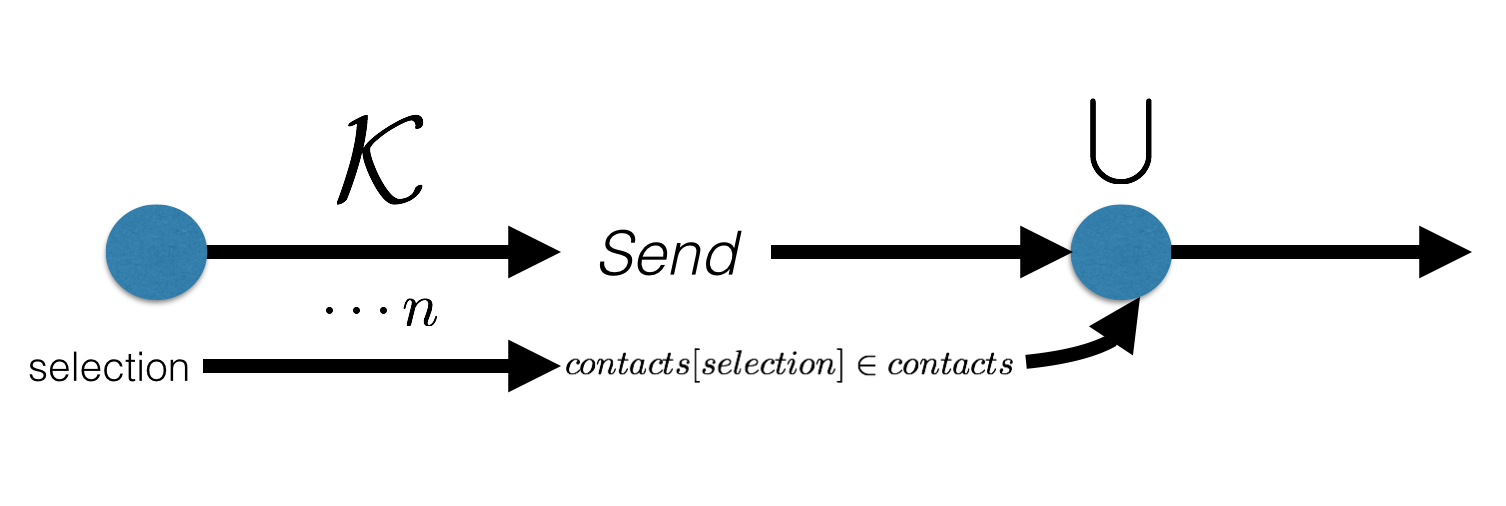
\includegraphics[width=\linewidth]{contactpickerpolicy}

\begin{lstlisting}
let cur_contact = ref None

let handle_s n =
  current_contact := Some n

let handle_b () =
  case (!cur_contact) of
    | None -> ()
    | Some n -> send net (declassify (nth contacts n))

let onCreate () = 
  new_button id_b "Send contact";
  install id_b handle_b;
  new_spinner id_s (declassify (length contacts)) "Contacts";
  install id_s handle_s
\end{lstlisting}

In this case, the program manipulates a free variable containing a
private list of contacts, the type of which is \code{list(string)}.
The program creates a spinner whose values range over the list of
contacts, and creates a button which the user can click.  The program
then repeatedly waits for the user to either select a new contact, or
presses a button to select the current contact.  The program first
checks to ensure that some contact has been selected.

\begin{displaymath}
  \begin{array}{c}
    (\code{id_b}, ()) \wedge \tlast{\code{id_s}}{n}
    \trelease
    \code{nth contacts n}
  \end{array}
\end{displaymath}

\subsection{Bump app: a bunch of checkboxes}

This is an application that has a button and a certain set of
contacts.  We want to reason that whenever the attacker can infer the
phone number or email, it was proceeded by a release of the data,
which means that the email checkbox went to one, and then the button
was clicked, without any intermediary changes in the email checkbox
value (or number..).

\begin{lstlisting}
let email_release = ref false
let phone_release = ref false

let handle_b =
  if email_release && phone_release then
    send net (declassify email + "|" + declassify phone)
  else if email_release
    send net (declassify email)
  else if phone_release
    send net (declassify phone)

let handle_c r v =
  r := v
    
let onCreate () = 
  new_checkbox id_e "Email?";
  install id_e (handle_c email_release);
  new_checkbox id_ph "Phone #?";
  install id_ph (handle_c phone_release);
  new_button id_b "Send";
  install id_b handle_b
\end{lstlisting}

The policy in this case is the following:

Whenever the button is clicked (a \code{send} event is handled), if
the email box is currently selected, then add that to the current
knowledge.  If the number box is selected, then add that to the
current knowledge.

\begin{displaymath}
  \begin{array}{c}
    \left[(\code{id_b}, ()) \wedge \tlast{\code{id_e}}{\strue}
    \trelease \code{email}\right] \\
    \wedge 
    \left[(\code{id_b}, ()) \wedge \tlast{\code{id_ph}}{\strue}
    \trelease \code{phone}\right] \\
  \end{array}
\end{displaymath}  

% \begin{array}{l}
% \text{id\_send} \wedge last(\text{id\_numberBox}) = 1 ~~ Releases ~~ value(number)
% \end{array}
% \end{displaymath}

% \begin{displaymath}
% \begin{array}{l}
% \text{id\_send} \wedge last(\text{id\_emailBox}) = 1 ~~ Releases ~~ value(email)
% \end{array}
% \end{displaymath}

\subsection{Toggling resolution of collected data}

Many apps include access to time varying data sources, such as
location information.  The user may feel uncomfortable revealing their
fine grained information to the application, but may be okay revealing
their location when they allow it: e.g., when they check a box.
Because of this, the app might present a configuration option to the
user that allows them to toggle the data collection between fine
grained and coarse grained information.  As an example, a restaurant
recommendation might have options that give ads to the user based on
their city, but might also recommend restaurants in their
neighborhood.

One example implementation might use a checkbox to select whether the
app should be sharing fine grained information, and collect
information only at times when the checkbox is checked:

\begin{lstlisting}
type prec = Truncate | Full
let prec_policy = ref Truncate

let handle_r v =
  if v = 0 then
    prec_policy := Truncate
  else if v = 1 then
    prec_policy := Full

let handle_loc loc = 
  case !prec_policy of
    Truncate -> send net (declassify (truncate loc))
  | Full -> send net (declassify loc)
  
let onCreate () = 
  new_radio_buttons id_r
    [(0, "Truncate"); (1, "Full precision")];
  install id_r handle_r;
  install loc handle_loc
\end{lstlisting}

\begin{displaymath}
  \begin{array}{c}
    [\forall x . (\code{loc}, x) \wedge \tlast{\code{id_r}}{0} \trelease
    \code{truncate}~x]
    \\
    \wedge 
    [\forall x . (\code{loc}, x) \wedge \tlast{\code{id_r}}{1} \trelease x]
    \\
    \wedge
    [\forall x . (\code{loc}, x) \wedge (\nexists y . \tlast{\code{id_r}}{y}) \trelease
    \code{truncate}~x]
  \end{array}
%  \begin{array}{l}
%last(\text{id\_checkbox}) = 1 ~~ Releases ~~ value(last(\text{location}))
%\end{array}
\end{displaymath}

\subsection{Geofencing app}

This is an app that responds to requests for the collected
information, as long as the user is within a certain designated area.

\begin{lstlisting}
let last_loc = ref (0, 0)

let handle_net_in () =
  if in_bounds (!last_loc) then
    send net last_loc

let handle_loc loc =
  if (can_satisfy(loc))
    last_loc := loc
  
let onCreate = 
  install loc handle_loc;
  install net_in handle_net_in
\end{lstlisting}

\begin{displaymath}
  \begin{array}{c}
    \forall x . (\code{net_in}, ()) \wedge \tlast{\code{loc}}{x}
    \wedge (\textit{in\_bounds}~x) \trelease x
  \end{array}
\end{displaymath}

\jeff{The above policy assumes we can check the \emph{in\_bounds}
  predicate and that it's the same as \code{in_bounds}. A bit yucky
  and perhaps not interesting.}

\subsection{Continuous/intermittent location app}

\begin{lstlisting}
let last_loc = ref (0, 0)

let continuous = ref false

let handle_loc loc =
  last_loc := loc;
  if (!continuous)
    send net loc

let handle_c v =
  continuous := v

let handle_b () =
  send net (!last_loc)

let onCreate =
  install loc handle_loc;
  new_checkbox id_c "Continuous map update?";
  install id_c handle_c;
  new_button id_b "Show my location";
  install id_b handle_b
\end{lstlisting}

\begin{displaymath}
  \begin{array}{c}
    [\forall x . (\code{loc}, x) \wedge \tlast{\code{id_c}}{\strue}
    \trelease x] \\
    \wedge
    [\forall x . (\code{id_b}, ()) \wedge \tlast{\code{id_c}}{\sfalse}
    \wedge \tlast{\code{loc}}{x} \trelease x] \\
    \wedge
    [\forall x . (\code{id_b}, ()) \wedge (\nexists y . \tlast{\code{id_c}}{y})
    \wedge \tlast{\code{loc}}{x} \trelease x] \\
  \end{array}
\end{displaymath}

\section{Formalism}
\label{sec:formalism}

In this section we deal with two formalisms, the first is the
formalism of the operational sematnics for our progrmaming language.
Our language is based around a reactive semantics that allows handling
messages on a message queue.  Programs evolve by sending messages on
channels, and responding to messages sent on channels.  In this way,
programs can respond to various user input (GUI elements) and also
communicate back and forth with third parties (via channels that are
handled over the network).

Next, we give the semantics for our variant of epistemic temporal
logic.  Our epistemic temporal logic works on sets of program traces,
which are agnostic to the core programming language, though we
consider the semantics presented here.  We give a models relation,
which relates sets of traces to valid well formed formulas, and in
subsequent sections we show that the epistemic semantics presented
here can encode definitions of noninterference from the literature.

\begin{figure}[t]
  \begin{displaymath}
    \begin{array}{lrcl}
      \hbox{prims} & \xv & ::= & n \mid f(\xv_1, \ldots, \xv_i)  \\
      \hbox{values} & v & ::= & \xv \mid \loc \mid \lambda x.e \\
      % \mid \sch
      \hbox{exprs} & e & ::= &
      v
      \mid x
      \mid e_1~e_2
      \mid \sref{e}
      \mid \sassign{e_1}{e_2}
      \mid \;\sderef{e} \\
      && \mid & \scase{e}{\aset{f(x_{i1}, \ldots, x_{ij}) \rightarrow
          e_i}_{i\in 1..k}} \\
      && \mid & \sinstall{\sch^{\{i,s,u\}}}{e}
      \mid \ssend{\sch^{\{o,s,u\}}}{e}
      \mid \sdeclassify{e} \\
      \hbox{constrs} & f & ::= &
      \sfmt{none} \mid \sfmt{some} \mid \sunit \mid \cdots \\
      \hbox{channels} & \sch^{\{i,o,s,u\}} & ::= & \sfmt{netin} \mid \sfmt{netout}
      \mid \cdots \\
%      \hbox{types} & \typ & ::= & \tint \mid \sch(\typ_1, \ldots, \typ_i) \\ \\
    \end{array}
  \end{displaymath}    

  % \begin{displaymath}
  %   \begin{array}{ll}
  %     \loc \in \textit{Locations}
  %   \end{array}
  % \end{displaymath}
    
  \begin{displaymath}
    \begin{array}{rcll}
      \Sigma & = & (M, \sigma, H, S, i) & \hbox{State} \\
      \evt & : & \sch \times p \times i  & \hbox{Message} \\
      M, t & : & \evt ~ \textit{list} & \hbox{Message queue, trace}\\
      \sigma & : & \loc \rightarrow v & \hbox{Heap} \\
      H & : & \sch \rightarrow \lambda x.e & \hbox{Handler map} \\
      S & : & \sch \rightarrow i \rightarrow v & \hbox{Secrets}
    \end{array}
  \end{displaymath}
  \caption{Source language syntax and semantic definitions}
  \label{fig:lang}
\end{figure}

We formalize our security policies for the source language shown in
Figure~\ref{fig:lang}. \emph{Primitives}~$xv$ are those values that
may appear in events (e.g., button clicks, network sends) in the
message queue. Primitives consist of integers and terms built from
constructors $f$, e.g., \sfmt{none}, \sfmt{some}, etc. In
Section~\ref{sec:examples} we used the unit value $()$, which we can
encode as a nullary constructor $\sunit$.

\emph{Values}~$v$ consist of primitives, heap locations~$\loc$, and
lambdas. \emph{Expressions}~$e$ are mostly standard, and include
values, variables~$x$, function applications~$e_1~e_2$, memory
allocation~$\sref{e}$, assignment~$\sassign{e_1}{e_2}$, and
dereference~$\sderef{e}$.  Expressions also includes the pattern
matching form \sfmt{case}, which evaluates its first argument to some
constructed term and then evaluates whichever rule matches. We omit
standard conditionals, since they can be encoded as two nullary
constructors $\strue$ and $\sfalse$ with pattern instead of the
standard $\sfmt{if}\ldots\sfmt{then}\ldots\sfmt{else}$ form.

The last three expression forms are particular to our
setting. $\sinstall{\sch}{e}$ installs $e$ (which must evaluate to a
lambda) to receive messages on a channel $\sch$; as we saw
previously, channels may include the network (\sfmt{netout},
\sfmt{netin}), channels for GUI events such as button clicks, and
channels for location updates. The network channels are distinguished
in the sense that the adversary is assumed to have access to them,
whereas all other channels are assumed to be private to the user.

The expression $\ssend{\sch}{e}$ sends $e$ (which must evaluate to a
primitive) over a channel. Finally, $\sdeclassify{e}$ marks an
expression the programmer intends to send over the network.


\begin{figure*}[t]
  \small
  \begin{displaymath}
    \begin{array}{c}
      \multicolumn{1}{l}{
        \framebox{$e, \Sigma_1 \sreduce v, \Sigma_2$}
      }
      \\ \\

      \infer[RVal]
      { }
      { v, \Sigma \sreduce v, \Sigma }

      \qquad

      \infer[RApp]
      {
        e_1, \Sigma_1 \sreduce (\lambda x.e_3), \Sigma_2 \\
        e_2, \Sigma_2 \sreduce v_1, \Sigma_3 \\\\
        \aset{x\mapsto v_1}e_3, \Sigma_3 \sreduce v_2, \Sigma_4
      }
      { e_1\;e_2, \Sigma_1 \sreduce v_2, \Sigma_4}

      \qquad

      \infer[RRef]
      {e, \Sigma_1 \sreduce v, \Sigma_2 \\
        \loc \not\in \dom(\Sigma_2.\sigma) \\\\
        \sigma' = \Sigma_2.\sigma[\loc\mapsto v]
      }
      {\sref e, \Sigma \sreduce \loc, \Sigma_2[\sigma \mapsto \sigma']}

      \qquad

      \infer[RAssign]
      {e_1, \Sigma_1 \sreduce \loc, \Sigma_2 \\
        \loc \in \dom(\Sigma_2.\sigma) \\\\
        e_2, \Sigma_2 \sreduce v, \Sigma_3 \\
        \sigma' = \Sigma_2.\sigma[\loc \mapsto v]
      }
      {\sassign {e_1} {e_2}, \Sigma_1 \sreduce
        v, \Sigma_2[\sigma \mapsto \sigma']}

      \\ \\

      \infer[RDeref]
      {e, \Sigma_1 \sreduce \loc, \Sigma_2 \\
       \Sigma_2.\sigma(\loc) = v}
      {\sderef e, \Sigma_1 \sreduce v, \Sigma_2 }

      \qquad

      \infer[RCase]
      {e_1, \Sigma_1 \sreduce f(v_1, \ldots, v_n), \Sigma_2 \\
        \aset{x_i\mapsto v_i}_{i\in 1..n}e_2, \Sigma_2 \sreduce v, \Sigma_3
      }
      {\scase{e_1}{\aset{\ldots, f(x_1, \ldots, x_n) \rightarrow
          e_2, \ldots}}, \Sigma_1 \sreduce v, \Sigma_3}
      \\ \\

      \infer[RInst]
      {
        e_1, \Sigma_1 \sreduce (\lambda x.e_2), \Sigma_2 \\
        H' = \Sigma_2.H[\sch \mapsto \lambda x.e_2]
      }
      {
        \sinstall \sch {e_1}, \Sigma_1 \sreduce \sunit, \Sigma_2[H
        \mapsto H']
      }

      \qquad

      \infer[RSend]
      { e, \Sigma_1 \sreduce \xv, \Sigma_2 \\
        M' = \Sigma_2.M, (\sch, \xv)
      }
      { \ssend \sch e, \Sigma_1 \sreduce \sunit, \Sigma_2[M \mapsto M']}

      \qquad

      \infer[RDeclassify]
      {e, \Sigma_1 \sreduce v, \Sigma_2}
      {\sdeclassify{e}, \Sigma_1 \sreduce v, \Sigma_2}

      \\ \\

      \multicolumn{1}{l}{
        \hbox{\textit{In machine state $\Sigma_1$, expression $e$ reduces to
          value $v$ and updates machine state to $\Sigma_2$.}}
      }

      \\ \\ 

      \multicolumn{1}{l}{
        \framebox{$\Sigma_1 \treduce^{\evt} \Sigma_2$ \hbox{ and } $S
          \judge e \sreduce t$}
      }
      \\ \\

      \infer[THandle]
      { \Sigma_1.M = (\sch^{\{i,s,u\}}, \xv,i), M' \\
        \Sigma_1.H(\sch) = \lambda x.e \\\\
        \Sigma' = \Sigma_1[M\mapsto M'] \\
        d = e \aset{x \mapsto \xv}, \Sigma' \sreduce v', \Sigma_2 \\
      }
      { \Sigma_1 \treduce^{\cdot} \Sigma_2 [i \mapsto \Sigma_1.i
          + 1] }

      \qquad

      \infer[TOutput]
      { \Sigma.M = (\sch^o,p,i), M' \\\\
        \Sigma' = \Sigma[M\mapsto M'][i\mapsto \Sigma.i + 1]
      }
      { \Sigma \treduce^{(\sch^o, p, \Sigma.i)} \Sigma'}

      \\ \\ 

      \infer[TInput]
      { \Sigma' = \Sigma[M \mapsto \Sigma(M) @ (\sch^i , p, \Sigma.i)][i\mapsto \Sigma.i + 1] \\\\
        \sch^i \in \dom(\Sigma.H) %% This rule needs to be ammended to
                                %% mention the set of input channels,
                                %% but how?  Do I simply need to
                                %% parameterize the whole inference
                                %% rule by some set of input channels?
                                %% In reality it's like we need to
                                %% label inputs, outputs, and
                                %% auxiliary channels with distinct
                                %% subscripts in the program text.
      }
      { \Sigma \treduce^{(\sch^i , p, \Sigma.i)} \Sigma' }

      \qquad


      \infer[TLookupSecret]
      { \Sigma.M = (\sfmt{getsecret},\sch^s,i), M' \\\\
        \Sigma' = \Sigma[M\mapsto M' @ (\sch, \Sigma.S(\sch)(\Sigma.i))][i\mapsto \Sigma.i + 1]
      }
      % I don't know what to put here..
      { \Sigma \treduce^{(\sch, \Sigma.S(\sch)(\Sigma.i), \Sigma.i)} \Sigma'}
      
      \\ \\ 

      % I also don't know if this is right
      \infer[TProg]
      {
      \Sigma_0 = ([], \emptyset, \aset{\code{main} \mapsto e}, S , 0)
        \\\\ 
      \Sigma_i \treduce^{\evt_i} \Sigma_{i+1}
      \quad i \in [0..n]
      }
      { S \judge e { \sreduce \evt_0 \cdot \evt_1 \cdots \evt_n } }

      \\ \\

      \multicolumn{1}{l}{
        \hbox{\textit{Machine state $\Sigma_1$ steps to state $\Sigma_2$ generating
            message $\eta$, and given secret inputs $S$, program $e$
            generates \tr.}}
      }

    \end{array}
  \end{displaymath}
  \caption{Operational semantics}
  \label{fig:semantics}
\end{figure*}

\paragraph*{Semantics}

Figure~\ref{fig:semantics} gives an operational semantics for our
language. The semantics uses the definition of a \emph{state}~$\Sigma$
from Figure~\ref{fig:lang}. A machine state $(M, \sigma, H)$ include a
\emph{message queue}~$M$, a list of \emph{messages}~$\evt$, which are
channel, primitive pairs; a \emph{heap}~$\sigma$, which maps locations
to values; and a \emph{handler map}~$H$, which maps a channel name to
the function installed to handle events on that channel. We also write
$t$ for message queues that are \emph{traces} of externally visible
messages; more on this below.  To keep our semantics concise, we write
$\Sigma.X$ (where $X$ could be $M$, $\sigma$, or $H$) to mean the $X$
component of $\Sigma$. Similarly, we write $\Sigma[X\mapsto X']$ to
mean $\Sigma$ where the $X$ component has been replaced to $X'$.

The top portion of Figure~\ref{fig:semantics} defines big-step
judgments of the form $e, \Sigma_1 \sreduce v, \Sigma_2$, meaning
evaluating expression $e$ in state $\Sigma_1$ produces a value $v$ and
new state $\Sigma_2$. The first several rules are standard.
\textsc{RVal} evaluates a value to itself, without changing the
state. \textsc{RApp} evaluates $e_1$ to a lambda, evaluates $e_2$ to
a value, and then evaluates the body of the lambda with the actual
argument substituted for the formal variable.

\textsc{RRef} evaluates $e$ to a value $v$, finds a fresh location
$\loc$ in the heap, and then evaluates to $\loc$, returning a state
where the heap maps $\loc$ to $v$. \textsc{RAssign} evaluates $e_1$
to a location $\loc$ and then updates the contents of
$\loc$. \textsc{RDeref} evaluates $e$ to a location and returns the
contents of that location. \textsc{RCase} evaluates $e_1$ to a
constructed term and then evaluates the matching expression with the
pattern variables $x_i$ replaced by the corresponding values
$v_i$. This rule is non-deterministic if there is more than one
matching pattern, but by convention we assume this does not occur.

\textsc{RInst} evaluates $e_1$ to a lambda and adds it as a handler
for channel $\sch$; the result value is the unit value
$\sunit$. \textsc{RSend} evaluates $e$ to a primitive $\xv$, and then
adds the message $(\sch, \xv)$ to the end of the message
queue. Finally, \textsc{RDeclassify} simply evaluates the expression;
this form has no run-time effect in the standard semantics.
\jeff{That seems weird---is there something we need to do to the
  semantics here?}

\paragraph*{Trace Generation}
As we saw in Section~\ref{sec:examples}, programs in our language
actually execute as a series of handlers that consume inputs and
produce outputs, quiescing in between each handler until a new input
arrives. The bottom part of Figure~\ref{fig:semantics} presents rules
that orchestrate this process.

The first three rules prove judgments of the form $\Sigma_1
\treduce^{\evt} \Sigma_2$, meaning the machine in state $\Sigma_1$
produces a new state $\Sigma_2$, possibly involving an action $\evt$
visible to either the user or the adversary.

\textsc{THandle} consumes a message $(\sch, \xv)$ from the front of
the message queue (recall \textsc{RSend} adds a message to the
\emph{back} of the message queue), looks up the handler for $\sch$,
and then invokes the handler, passing $\xv$ as its argument. Notice
that the handler is invoked as a big-step; thus, handler execution is
always atomic. \jeff{Say more?}  Running a handler is not an
externally visible operation, which is indicated by an empty
message $\cdot$ on the reduction arrow.

\textsc{TOutput} models the network, consuming a single message from
\sfmt{netout}. Since the message may be seen by the adversary, it
decorates the reduction arrow. Finally, \textsc{TInput} models an
input message coming into the system, either from the user or from the
adversary (on \sfmt{netin}). The rule non-deterministically chooses
some $\sch$ for which a handler is defined (recall by convention this
excludes \sfmt{netout}) and a value $p$, and sends $\sch$ the message
$p$. \jeff{What about ranges for $p$? Seems a bit icky to get into
  that, but otherwise our examples will break...} The message
decorates the reduction arrow because it is externally visible.

The last rule in the bottom right of Figure~\ref{fig:semantics},
\textsc{TProg}, proves a judgment of the form $e \sreduce t$, meaning
running the program $e$ produces a trace $t$ of externally visible
messages. This rule runs $e$ starting from the empty state, producing
a value $v$ that is discarded and an initial state $\Sigma_0$. It them
repeatedly reduces $\Sigma_i$ to produce a new state $\Sigma_{i+1}$,
possibly generating a message $\eta_0$. Then the trace $t$ produced is
the concatenation of the $\eta_i$; here empty messages $\cdot$ are
discarded from the concatenation. Notice that the length of the trace
$n$ is non-deterministic; in general, since these are reactive
programs, they can potentially run for an any number of steps as long
as additional input arrives.

\paragraph*{Differences between derivation and trace}

A derivation is an execution (repeated appliction of derivation rules)
to a program with some initial secret environment $S$.  We use $\pi$
to refer to a derivation in our semantics, and we use $\tr$ to refer
to a trace.  Our epistemic temporal logic talks about traces, which
are simply sequences of messages.  Going from a derivation to a trace
is a projection from the sequence of rules to the derivation to the
sequence of messages on top of the arrows, i.e., a fold followed by a
filter (of the empty messages).  In our notation we use the function
$trace(\pi)$ to refer to the trace corresponding to the derivation
$\pi$.

\paragraph*{Derivation extension} 

(When a trace $\tr_2$ extends $\tr_1$ in the operational sense.)

For a given derivation $\pi_1$, we say that $\pi_2$ extends $\pi_1$
($\pi_1 \rightarrow^\ast \pi_2$) if $\pi_2$ is the derivation obtained
by extending $\pi_1$ with the additional derivation $\Sigma_n
\rightarrow^\ast \Sigma_k$, and $\Sigma_n$ is the end of $\pi_1$.

Does the previous thing I said make sense?

If $\pi_1$ is: 

\begin{displaymath}
  \begin{array}{c}
    S \judge e \Downarrow \tr ~ \text{by} ~ \Sigma_i
    \rightarrow^{\eta_i} \Sigma_{i+1} ~ i \in [0..n]
  \end{array}
\end{displaymath}

And $\pi_2$ 

\begin{displaymath}
  \begin{array}{c}
    S \judge e \Downarrow \tr ~ \text{by} ~ \Sigma_i
    \rightarrow^{\eta_i} \Sigma_{i+1} ~ i \in [0..k]
  \end{array}
\end{displaymath}

Where $n \leq k$ and the first $n$ agree in $\pi_2$, then $\pi_2$
extends $\pi_1$.

\paragraph*{Definition of $\mathcal{M}(e)$} We frequently need to talk
about all of the traces that could be generated by the program (e.g.,
to reason about what an attacker could know with the $K$ modality in
our logic).  The notation $\mathcal{M}(e)$ refers to the set of
derivations that could be generated by the program $e$ if any initial
set of secrets was used.  I.e., it is the set $\bigcup_{S \in Secrets}
\{S \judge e { \sreduce t } \}$.

Type of $M(e)$: the type of M(e) is a set of derivations, not a set of
traces.  A trace is a sequence of messages, a deriviation includes the
actual machine states, which are needed to define other things (e.g.,
traditional noninterference).

Note that M(e) is something that depends on the semantics of the
programming language, while our definitions in ETL are not.  This
means that no matter what semantics we use, while the definition of
noninteference changes based on the programming langauge, our
definitions in ETL don't have to be.

%JF: We're abusing notation slightly here in using nonterminal in the
%"types" of things like M, but I think it's okay.

\section{Epistemic Temporal Logic Formalism}

We define a linear time epistemic logic, whose purpose is to describe
at what points in a system certain values an observer may ascertain.
In our logic, we assume that values are sent on channels, and that an
external observer (such as a server communicating with a client) may
observe a stream of values (such as writes to the internet).  By
watching a sequence of writes, an observer may infer values about what
secret values may have been.

\paragraph*{Secrets} In our formalism, we assume that a secret is a
time varying input to the program.  At each time step, a program may
read a value and do some computation with that value, potentially
leading to an information leak.

An information leak is any two executions of the program in which
different secret inputs lead to different secret outputs.  As a
running example we consider the following program (which we call
$e$):

\begin{lstlisting}
let main(secret) =
  send (net, secret mod 2)
\end{lstlisting}

This program accepts a secret input and then sends the output to the
\code{net} channel.  To give examples that use more human readable
names, we will say that Alice is running the program on her machine,
and provides the secret input (the value of the variable
\code{secret}).  We will say that Bob is ``listening'' on the other
end of the \code{net} channel.  In our semantics, we do not formally
model Bob as a third party, our epistemic judgements are given by
speaking about some set of channels which Bob can observe.  This is to
say, if Bob couldn't read from the \code{net} channel, then he would
never learn anything about Alice's secret inputs, because he would
never be able to read any output.  If Bob never sees any output of the
program, and doesn't have any extenal source telling him about Alice's
input (e.g., a spy, who tells Bob that Alice's input is actually 1),
he cannot reasonably conclude anything about the value of
\code{secret}.

Bob ``learns'' facts about the value of secret by watching the output
of Alice's program.  As she sends Bob input, he refines his belief
about what her secret input must have been.  For example, consider two
possible secret inputs, $0$ and $1$.  We have that:

\begin{displaymath}
  \begin{array}{c}
    \aset{secret \mapsto const(0)} \judge e \sreduce 0 \cdot \\
    \aset{secret \mapsto const(1)} \judge e \sreduce 1 \cdot
  \end{array}
\end{displaymath}

In the previous notation, we use the dot to indicate a partial trace
(in reality this would be the end of the program, but we could imagine
a program which generates more input).  In the first case, Alice
provides the secret input 0, but Bob doesn't know this.  However, Bob
sees the output is 0.  He then considers the other possibility, but
there is no other possibility, so then he (epistemically) concludes
that Alice must have provided the secret input 0 to the program.

Note that in the above, we used the \code{const} function to indicate
the stream that returns $0$ at any time.  In our formalism, we talk
about a series of timestamped (monotonically increasing) messages
appearing on channels.  In the programming languge semantics we model
time varying inputs as functions that are passed in the trace
generation judgement, but our epistemic logic speaks about values that
appear on streams at certain times agnostic from where they come from.
(This is to say that no matter what we choose to give time varying
inputs to programs, as long as the set of traces is the same,
isomorphic cosmetic changes in the semantics will not change the
semantics of the epistemic temporal logic formulas.)

An observer ``learns'' information by looking at the set of traces and
using epistemic reasoning to infer facts about what the secret inputs
to the program may have been.  Bob observes values that Alice sends
over the \code{net} channel from her program, but doesn't see anything
else about the execution of the program.  Therefore, when Bob sees
that Alice sends a $1$ on the \code{net} channel, Bob reasons
backwards and ascertains that the value Alice read from the
\code{secret} channel must have been an odd number.  Conversely, if
Bob reads a $0$ from the \code{net} channel, he reasons that Alice
must have read an even number.  If we view values on these secret
channels as secret inputs to the program, then we might view it as
bad, because (from an information theoretic perspective) Bob has
learned one bit of information about Alice's secret input to the
program $e$.

\paragraph{Execution traces}
Consider the above program $e$, the set of traces for the program is
$\mathcal{M}(e)$.  The program is finite and terminates, because the
program doesn't queue any handlers after the \code{main} function
ends.

Each execution in the program has this template:

\[
\Sigma_0 \rightarrow^{(secret,v,0)} \rightarrow \Sigma_1 \rightarrow^\cdot \Sigma_2 \rightarrow^{(net, v \% 2, 2)}
\]

Where $\Sigma_0$ is the initial configuration taken by injecting the
main function into the handler map as discussed previously.  The
nondeterministic input rule TInput allows us to input the value from
the secret stream (note that no other rules lead to further
reductions, and so we can unambiguously say that this must happen).
In our semantics, secrets are read off of time varying streams,
meaning that the value of \code{secret} at time 0 may be different
than the value of secret at some other time.

\paragraph{Noninterference for this example}

Noninterference is a property that essentially means: Bob learns
nothing about the input to the program.  This is to say, given the
output (trace generated by $e$ on the \code{net} channel) Bob cannot
discern between any secret input.

\begin{displaymath}
  \begin{array}{l}
    \forall \pi_1, \pi_2 \in M(e),
    trace(\pi_1) \equiv^{\{Bob\}} trace(\tr_2)
    \, \wedge \, \pi_1 \rightarrow^\ast \pi_1'
    \, \wedge \, \pi_2 \rightarrow^\ast \pi_2' \\
    \, \, \implies trace(\tr_1') \equiv^{\{Bob\}} trace(tr_2')
  \end{array}
\end{displaymath}

The 

%% Need to define trace extension as the set of trace suffixes
%% generated by taking the last thing in that trace and performing
%% closure over operational semantics

\paragraph{ETL defn of noninterference for this example}

%% ETL defn here and why it works

\paragraph{Relaxed noninterference for this example}

%% Standard trace-set based formulation of relaxed NI for this example

\paragraph{ETL relaxed NI for this example}

%% Encoding relaxed NI for this example in ETL

\paragraph{Multiple reads}

%% About time varying data inputs from streams

\paragraph{Protecting secret values until alice flips a bit}

%% Declassification policy with time varying data

%% XXX: write here about hiding a value 

\paragraph{A note on observational equivalence}

Consider the following program:

\begin{lstlisting}
let handle_spinner secret value = 
  sleep value
  send (net, 1)

let main(secret) =
  new_spinner id (handle_spinner secret) 5
\end{lstlisting}

Where sleep is a recursive function that waits some number of steps
based on the value given to function.  In the previous, we have
allowed the user to select up to five values by creating a new spinner
using the \code{new_spinner} function.  Consider the execution trace
of this program:

\[
\Sigma_0 \rightarrow^{(secret,v,0)} \Sigma_1 \rightarrow^{n \in
  \{1..5\}} \Sigma_2 \overbrace{ \rightarrow^\cdot \cdots
  \rightarrow^\cdot \Sigma_k}^\text{$O(n)$ times}
\rightarrow^{(net,1,k)}
\]

When an attacker looks at a trace of a program, they will only observe
the following trace:

\[
secret \judge e \Downarrow 1 \cdot
\]

(Note again that the dot above means that we are focusing on the point
in time in which the attacker sees the stream on the left side of the
dot.)  Note that while the user could have given any of the five
spinner inputs to the program, the set of spinner program outputs
would be the same:

\begin{displaymath}
\begin{array}{c}
\Sigma_0 \rightarrow^{(secret,v,0)} \Sigma_1 \rightarrow^{n \in
  \{1..5\}} \Sigma_2 \rightarrow^\cdot \Sigma_3 \rightarrow^\cdot \Sigma_4
\rightarrow^{(net,1,4)} \\ 
\Downarrow \\ 
secret \judge 1 \cdot \\ \\ 

\Sigma_0 \rightarrow^{(secret,v,0)} \Sigma_1 \rightarrow^{n \in
  \{1..5\}} \Sigma_2 \overbrace{ \rightarrow^\cdot \cdots
  \rightarrow^\cdot \Sigma_k}^\text{5 times}
\rightarrow^{(net,1,k)} \\ 
\Downarrow \\ 
secret \judge 1 \cdot
\end{array}
\end{displaymath}

(Note that in the above illustration, we have used the down arrow to
map the derivation generated by our operational sematnics to a trace.)

All of this is to say that all five executions of the program will be
observationally equivalent.  Potentially more interesting, consider
the alternative example of the slightly simpler program:

\begin{lstlisting}
let main(secret) =
  sleep secret
  send (net, 1)
\end{lstlisting}

By the same reasoning we have above, we have that for all $n$,
$\aset{secret\mapsto const(n)} \judge e \Downarrow 1 \cdot$.  This
means that program satisfies noninterference in an observational
sense.  This discussion highlights one advantage of ETL: reasoning
about observational equivalence happens based on traces, which relate
to the program via the operational semantics, but are not solely tied
to it.

It also may be unrealistic to think that the most recent example
exhibits noninterference.  In reality, Bob might be listening to Alice
(who provides her input $secret$) and can keep a timer of when she
initiates her connection to him, and then when she sends her output.
Assuming that the \code{sleep} function waits for a reasonable amount
of time, it may be possible for Bob to conclude the value of $secret$
by timing Alice's messsages.  In other words, while Bob sees only a
filtered version of the derivation generated by Alice (which also
contains various ``noops'' from the dots in the steps shown above), he
may infer something about the derivation from the timing.

Such timing channels have been particularly hard to diagnose and cure,
one simple solution is to model timing by adding an explicit step
index to messages sent by Alice (i.e., instrument the semantics so
that traces are always timestamped).  This is called the program
counter model of security \cite{pcmodel}, and not always correct for
other reasons (caching, multicycle insructions, etc...).

\begin{figure}[t]
  \begin{displaymath}
    \begin{array}{rcl}
      \phi, \psi & ::= &
      (\sch, \xv)
      \mid \top
      \mid \neg \phi
      \mid \phi \wedge \phi
      \mid \phi \vee \phi
      \mid \phi \tuntil \phi
      \mid \phi \tsince \phi
%      \mid \tnext \phi
      \\
      & \mid & \talways \phi
      \mid \tevent \phi
      \mid \forall x . \phi
      \mid \exists x . \phi
      \mid \tknows{\sch} \phi
      \mid \tatmost{\sch} \phi
    \end{array}
  \end{displaymath}    

  \begin{displaymath}
    \begin{array}{rcl}
      \tset, \tr, i \models (\sch, \xv) & \iff &
      \tr[i] = (\sch, \xv) \\

      \tset, \tr, i \models \ltrue \\

      \tset, \tr, i \models \neg \phi & \iff &
      \tset, \tr, i \not \models \phi \\

      \tset, \tr, i \models \phi \land \psi & \iff &
      \tset, \tr, i \models \phi \hbox{ and } \tset, \tr, i \models \psi \\

      \tset, \tr, i \models \phi \lor \psi & \iff &
      \tset, \tr, i \models \phi \hbox{ or } \tset, \tr, i \models \psi \\

%      \tset, \tr, i \models \tnext \phi & \iff &
%      \tset, \tr, (i+1) \models \phi \\

      \tset, \tr, i \models \talways \phi & \iff &
      \forall j ~.~ j \geq i \Rightarrow (\tset, \tr, j \models \phi) \\

      \tset, \tr, i \models \tevent \phi & \iff &
      \exists j ~.~ j \geq i \Rightarrow (\tset, \tr, j \models \phi) \\

      \tset, \tr, i \models \phi \tuntil \psi & \iff &
      \exists j ~.~ j \geq i \Rightarrow ((\tset, \tr, j \models \psi)
      \hbox{ and } \\
      & & \forall k ~.~ i \leq k < j \Rightarrow (\tset, \tr, k
      \models \phi)) \\

      \tset, \tr, i \models \phi \tsince \psi & \iff &
      \exists j ~.~ j \leq i \Rightarrow ((\tset, \tr, j \models \psi)
      \hbox{ and } \\
      & & \forall k ~.~ j < k \leq i \Rightarrow (\tset, \tr, k
      \models \phi)) \\

      \tset, \tr, i \models \forall x . \phi & \iff &
      \forall v. (\tset, \tr, i \models \aset{x\mapsto v} \phi) \\

      \tset, \tr, i \models \exists x . \phi & \iff &
      \exists v. (\tset, \tr, i \models \aset{x\mapsto v} \phi) \\

      \tset, \tr, i \models \tknows{\sch} \phi & \iff &
      \forall u \in \tset ~.~
      \tr_{\sch}[1..i] \cong u_{\sch}[1..i] \Rightarrow \\ & & 
        \tset, u, i \models
      \phi \\
%
%      \tset, \tr, i \models \tatmost{\sch} \phi & \iff &
%      \forall \phi' . (\phi' \Rightarrow \phi
%      \wedge \phi' \neq \phi) \Rightarrow \neg\tknows{\sch} \phi
%      \\

      \tset, \tr, i \models \tatmost{\sch} \phi & \iff &
      \forall u \in \tset ~.~
      \tr_{\sch}[1..i] \not\cong u_{\sch}[1..i] \Rightarrow \\ & & 
        \tset, u, i \models \phi \\


      % \tset, \tr, i \models \tposs \phi & \iff &
      % \exists \tr' \in \tset ~.~
      % \tr[1..i] \cong \tr'[1..i] \Rightarrow \\ & & \tset, i, \tr' \models
      % \phi \\

    \end{array}
  \end{displaymath}

  \begin{displaymath}
    \begin{array}{rcl}
%      \phi \tthen \psi & \equiv & \psi \tsince \phi \\
      \tlast{\sch}{\xv} & \equiv &
      ((\neg \exists x . x \neq v \wedge (\sch, x)) \tsince (\sch, v)) \\
      \tset, t \models \phi \trelease v & \equiv &
      \tset, t, 0 \models \talways (\phi \Rightarrow (\exists y . \tatmost{\code{net}} (v = y)))
    \end{array}
  \end{displaymath}
  
  \caption{Epistemic temporal logic semantics and notation.}
\end{figure}

\begin{figure}[t]
  \begin{tabular}{ll}
     \textbf{A1.} & All instances of axioms and rules of predicate logic \\
     \textbf{A2.} & $\tknows{\sch} (\alpha \Rightarrow \beta) \Rightarrow (\tknows{\sch} \alpha \Rightarrow \tknows{\sch} \beta)$ \\
     \textbf{A3.} & $\tatmost{\sch} (\alpha \Rightarrow \beta) \Rightarrow (\tatmost{\sch} \alpha \Rightarrow \tatmost{\sch} \beta)$ \\
     \textbf{A4.} & $\tknows{\sch} \alpha \Rightarrow \alpha$ \\
     \textbf{A5.} & $\tatmost{\sch} \alpha \Rightarrow \neg \tknows{\sch} \alpha$ if $\alpha$ is not a validity \\
     \textbf{R1.} & From $\alpha$ infer $\tknows{\sch} \alpha \mathrel\wedge \tatmost{\sch} \alpha$.
  \end{tabular}
  \caption{A sound deductive system}
\end{figure}

\begin{figure}[t] 
  \begin{displaymath}
  \infer[KAM]
      {
        \mathrel\tatmost{\sch} \phi  \\
        \psi \Rightarrow \phi  \\
        \phi \text{~is not a validity}
      }
      {
        \neg \mathrel\tknows{\sch} \psi
      }
  \end{displaymath}
  \caption{An admissible inference rule}
\end{figure}


\subsection{Epistemic Temporal Logic}


We now discuss the formula langauge, which we present in
Figure~\ref{fig:sourcelang}.  Our formulas allow specification of
security policies for programs which include private inputs, and allow
modalities for time ($\lozenge$, $\square$, and $U$) and knowledge
($K$ and $L$).  The temporal modalities have their usual
interpretation ($\lozenge \phi$ means ``in the future $\phi$'',
etc...), but the epistemic modalities $K$ and $L$ allow us to reason
about attacker knowledge as in \cite{Balliu:11}.  As in their system,
$K \phi$ means ``in \emph{all} observationally equivalent states,
$\phi$ holds,'' and $L \phi$ means ``in \emph{some} observationally
equivalent state, $\phi$ holds.''

For example, consider the following program, which generates $secret$
ones along the output, before generating an infinite stream of zeros.

\begin{lstlisting}
let rec 
\end{lstlisting}

The set of traces generated by the program is shown in
\ref{fig:traces-example}.  Notice that the as the program continues
producing output, the adversary continues to learn different
predicates on the value of \code{secret}.  Namely, at each point that
the program writes a new $1$ onto the output channel, the attacker
learns that \code{secret} is greater than or equal to the number of
ones seen so far (because, in every observationally equivalent trace
it is true that \code{secret} $\geq len($\code{net}$)$).  Once the
attacker sees a zero, they know that \code{secret} $= n$, where n is
the number of values seen.  This is because there is only a single
trace in which $n$ ones will be written.

\begin{figure}
  \centering
  \begin{tabular}{cccccccc}
    \multicolumn{1}{ c| }{$x = 0$} & 0 & 0 & 0 & 0 & 0 & 0 & $\cdots$ \\
    \multicolumn{1}{ c| }{$x = 1$} & 1 & 0 & 0 & 0 & 0 & 0 & $\cdots$ \\
    \multicolumn{1}{ c| }{$x = 2$} & 1 & 1 & 0 & 0 & 0 & 0 & $\cdots$ \\ \cline{4-5} 
    \multicolumn{1}{ c| }{$x = 3$} & 1 & 1 & \multicolumn{1}{ |c| }{1} & \multicolumn{1}{ |c| }{0} & 0 & 0 & $\cdots$ \\ \cline{5-5} 
    \multicolumn{1}{ c| }{$x = 4$} & 1 & 1 & \multicolumn{1}{ |c| }{1} & 1 & 0 & 0 & $\cdots$ \\
    \multicolumn{1}{ c| }{$x = 5$} & 1 & 1 & \multicolumn{1}{ |c| }{1} & 1 & 1 & 0 & $\cdots$ \\
    \multicolumn{1}{ c| }{$x = 6$} & 1 & 1 & \multicolumn{1}{ |c| }{1} & 1 & 1 & 1 & $\cdots$ \\ \cline{4-4}
    \vdots &   & \multicolumn{3}{ c }{ $K (x \geq 3)$} & & \\
  \end{tabular}
  \caption{Trace based evolution of program XXXXXXXXX}
  \label{fig:traces-example}
\end{figure}

On top of the logic, we add the ability to reason about
declassification streams: $events(c)$ in the $exp$ form generates the
current set of declassification events on channel $c$ as run by the
semantics (in a configuration $\langle p , Cvm , Dc , Sigma \rangle$,
this is $Dc(c)$).  This gives us the ability to write formulas that
speak about GUI channels as declassification channels for private
information (which show up in the form of $secret(x)$).

\subsection{Definition of models relation}

Figure~\ref{fig:models-rel} gives the definition of the models
relation for a given trace and index into that trace, with respect to
a set of other traces.  The relation

\[
\mathcal{T}, (trace, n) \models \phi
\]

Says that, within the set of traces $\mathcal{T}$, a given trace
satisfies $\phi$ at index $n$.  Consider again the trace set from
Figure~\ref{fig:traces-example}.  Consider the case $x = 3$, in the

A \emph{program} models a formula if every trace in the program
satisfies the formula:

\[
\mathcal{P} \models \phi \iff \forall tr \in Tr(\mathcal{P}). \, Tr(\mathcal{P}),(tr,0) \models \phi
\]

\begin{figure}
  \begin{displaymath}
    \begin{array}{rcl}
      rcon & ::= &
      last(id) = ( v_1 , \dots , v_n ) \mid rcon \wedge rcon \\ 
      & \mid & rcon \lor rcon \mid \exists x ~.~ rcon
      \\ \\
      \phi & ::= & \forall x : \tau ~.~ \phi \mid op (v_1 , ... , v_n) = op (v_1 , ... , v_n) \\
      & \mid & value(op (v_1 , ... , v_n))
      \\ \\
      policy & ::= & rcon ~~ Releases ~~ \phi(secret)
    \end{array}
  \end{displaymath}    
  \caption{Release conditions and policies}
  \label{fig:rcons}
\end{figure}

\begin{figure}
  \begin{displaymath}
    \begin{array}{rcl}

      \tr, i \modelsrcon last(id) = ( v ) & \iff &
      \tr[i] = (id, v) \\

      \tr, i \modelsrcon last(id) = ( v ) & \iff & 
      \exists j ~.~ j \leq i \Rightarrow (\tr, j \modelsrcon last(id) = ( v ) and \\
      & & \forall k ~.~ i \leq k \Rightarrow (\tr, k \not \modelsrcon last(id) = ( v )) \\

      \tr, i \modelsrcon rcon_1 \wedge rcon_2 & \iff & 
      \tr, i \modelsrcon rcon_1 \hbox{ and } \tr, i \modelsrcon rcon_2 \\
      
      \tr, i \modelsrcon rcon_1 \lor rcon_2 & \iff & 
      \tr, i \modelsrcon rcon_1 \hbox{ or } \tr, i \modelsrcon rcon_2 \\

      \tr, i \modelsrcon \exists x ~.~ rcon & \iff & 
      \hbox{ for some } v, \tr, i \modelsrcon \aset{rcon \mapsto v} \\


    \end{array}
  \end{displaymath}
  \caption{A trace satisfies a release condition}
\end{figure}

\subsection{Release policies}

We now define the release conditions for information in programs.  Our
knowledge release definition ensures that programs only leak
information in accordance with declassification policies dictated by
constraints on GUI inputs, and that when knowledge is released, the
attacker learns at most what the policy allows them to learn.  We use
ideas from gradual release \cite{Askarov:2007} and epistemic temporal
logic to define our security condition \cite{Ahmad:13}.  While gradual
release allows us to define when knowledge can grow, it does not allow
us to say how (by how much) it can grow.  Epistemic logic allows us to
say by how much knowledge should be allowed to grow, but does not
admit an enforcement mechanism.

\subsubsection{Defining user actions}

We first define when an attacker is allowed to learn more knowledge.
Informally, a policy says that after some sequence of GUI inputs, an
attacker can learn some knowledge about a secret input.

All of our example programs have release conditions that are of this
form: if some sequence of user inputs happens, then some knowledge is
allowed to be released.  If the program takes a step, and no
additional knowledge has been released by a user action, then it
should stay the same.

The user takes some sequence of actions and a release event is allowed
to occur.  We formally define the grammar for release conditions as
$rcon$ in Figure~\ref{figure:rcons}.

%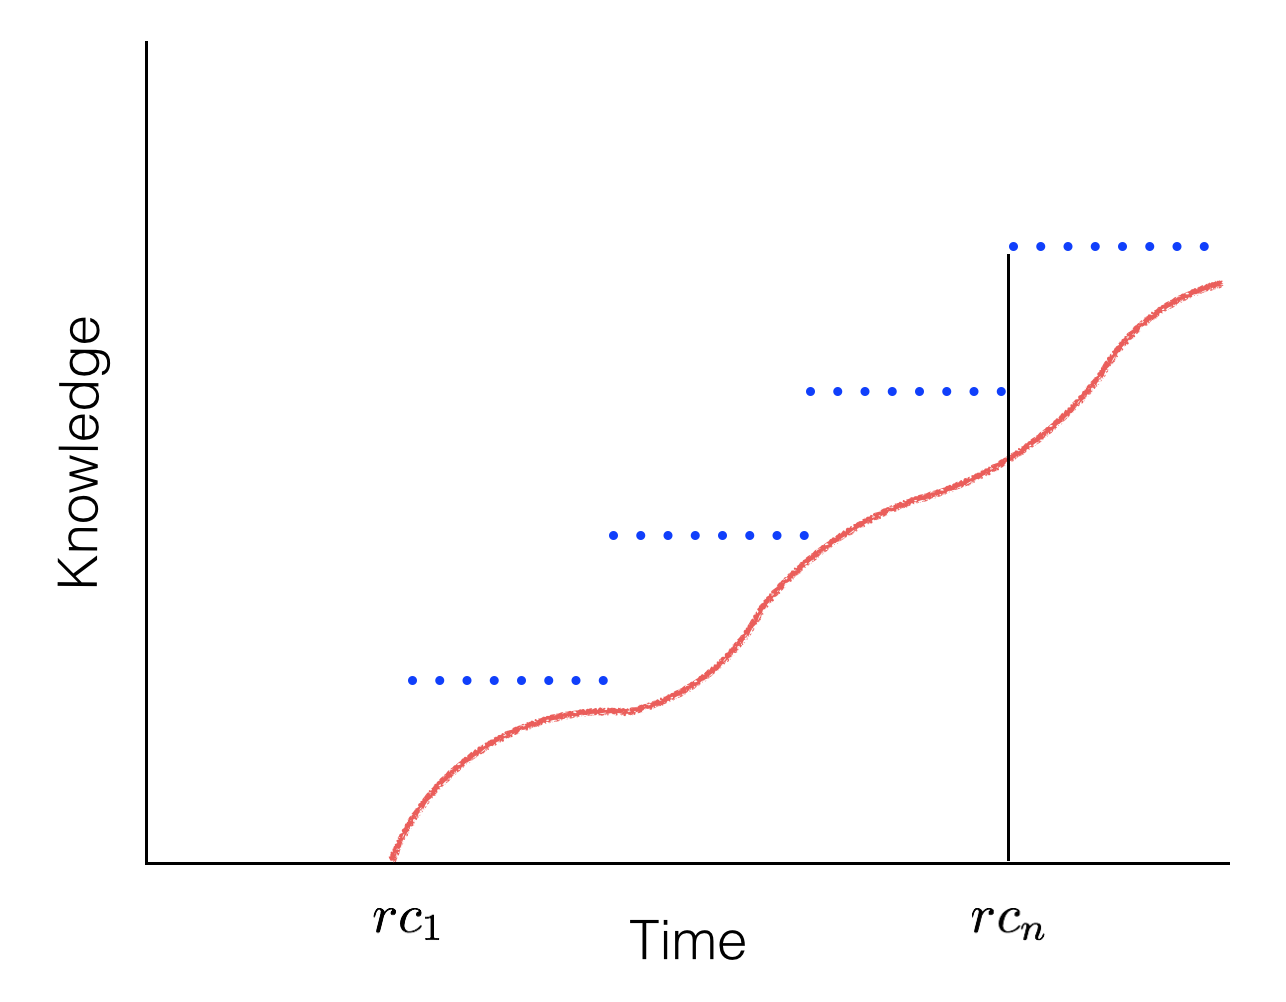
\includegraphics[width=\linewidth]{release-graph}


We now give a release semantics relation with respect to a set of
release policies $\pset$.  The release policies describe the
conditions under which information is allowed to be released from the
program to the attacker, which observes the program execution by
watching subsequent outputs on the net channel.  At any given time in
the program execution, there is a \emph{current} policy $\phi$, which
describes a maximum bound on the information which can be released at
the current time.  If the program releases more information than
$\phi$ allows, it violates the policy.


\section{Proofs}

Consider that we have a program $P$, such that $P$ can be assigned a
type for some $\Gamma$ in our type system.  Now consider that there
are no instances of \code{declassify} in the program, and we have an
empty release environment (i.e., $\pset = \emptyset$).  Under this
circumstance, we should see an analogue to noninterference.  The
typical statement of noninterference is based on a batch execution
style, but instead of a batch execution model, we assume that the
program can execute and that the attacker can observe runs.  Instead
of noninterference, our program satisfies a property called
observational determinism.

We define various notational conveniences: 

\begin{displaymath}
  \begin{array}{c}
    h_{id}(\Sigma) = id ~~ \text{where} ~~ \Sigma(M) = (id,v),M'
  \end{array}
\end{displaymath}

\begin{displaymath}
  \begin{array}{lll}
    h_{curr}(\Sigma) = e \aset{x \mapsto v} & ~~ \text{where} ~~ & \Sigma(M) = (id,v),M' \\
    & ~~\text{and}~~ & \Sigma(H)(id) = \lambda x . e
  \end{array}
\end{displaymath}

$M_{new}$ is the set of new messages written to the queue after a
given handler runs.

\begin{defn}[Low observational determinism]
  For any program $P$, which contains no instances of the
  \code{release} expression.  Consider a trace $\tr_1$ that starts
  from the initial configuration $\Sigma = (P, \emptyset,
  [(\code{onCreate},())])$.  Consider any index $i$ into $\tr_1$.  If
  is always the case that we can find $\tr_2$ and $k$ such that
  $\tr_1[1..i] \equiv_{\Gamma^{GUI}} \tr_1[1..k] \implies \tr_1[1..i]
  \equiv_{net} \tr_2[1..k]$ for all initial values $secret$, then we
  say that $P$ satisfies observational determinism.
\end{defn}

\begin{lem}[High effecting handlers do not queue any low handlers]
  For any well typed program $P$, and any configuration $\Sigma$ from
  the initial configuration, if $\Gamma(h_{id}) = H , \tau$, then for
  all new messages $\eta \in M_{new}$ generated by reducing
  $h_{curr}$, we will have that $\Gamma(id(\eta)) = H$.
\end{lem}

\begin{proof}
  Consider any configuration $\Sigma$, and now consider any expression
  $h_{curr}$.  By assumption $h_{curr} : H , \tau$.  Now use induction
  on the derivation of the typing judgement to prove the lemma.  There
  are a few cases:
  \begin{itemize}
  \item \code{ESend}: We know by assumption that $e$ has a high effect
    label.  We have that $\ssend{id~v} : H , H$, by hypothesis for
    some $id$, and have that $\Gamma(id) = H$ by the premise of the
    \code{ESend} rule.
  \item \code{EApp} and \code{EIf} Follow from noting that since the
    effect label is high, all of the subexpressions must also have
    high effect labels (because of $\sqcup$) and invoking the
    induction hypothesis.
  \item The rest of the cases follow trivially since they don't make
    any updates to the message queue.
  \end{itemize}
\end{proof}

\begin{lem}[Low typed expressions do not read from high parts of the
  store]
\end{lem}

\begin{proof}
  Induction on typing derivation:
  \begin{itemize}
  \item{EVal} By assumption the expression has a low type, the only
    case that would have a high value is a high variable, which is
    disallowed by the \code{VVar} rule.
  \end{itemize}
\end{proof}

\begin{lem}[Low typed expressions ]
\end{lem}

\begin{proof}
  Induction on typing derivation:
  \begin{itemize}
  \item{EVal} By assumption the expression has a low type, the only
    case that would have a high value is a high variable, which is
    disallowed by the \code{VVar} rule.
  \end{itemize}
\end{proof}

\begin{lem}[High effecting handlers do not affect low portions of the
  store]
  For any well typed program $P$, and any configuration $\Sigma$ from
  the initial configuration, if $\Gamma(h_{id}) = H , \tau$, and if
  $\Sigma \treduce^{\cdot} \Sigma'$ after reducing $h_{curr}$, for all
  locations $\loc \in dom(\sigma)$ such that $\Gamma(\loc) = L$,
  $\Sigma(\sigma)(\loc) = \Sigma'(\sigma)(\loc)$.
\end{lem}

\begin{proof}
  Proof: similar to above, induction on typing deviation.  The only
  rule which writes to the store is \code{EAsgn}.  By assumption and
  $\sqcap$ we know that the type on $e_1$ is also high.  Assuming that
  $e_1$ contains any subexpressions which are low variables leads to a
  contradiction via inversion of the typing rules for values.  The
  rest of the rules follow by induction.
\end{proof}

\begin{thm}
  For any program $P$ which can be assigned a type according to our
  typing judgement, $P$ satisfies low observational determinism.
\end{thm}

\begin{proof}
  Consider any run of $P$, whose trace is $\tr_1$.  Consider any
  arbitrary index into $\tr_1$, call it $i$.  We wish to prove that
  for any other run of $P$, $\tr_2$ where the initial secret is
  different, then we have that $\tr_1 \equiv_{net} \tr_2$ for at least
  $i$ steps.
  
  We now construct $\tr_2$ which has the desired properties.  Take any
  value of the secret input not equal to that in $\tr_1$ and obtain
  the initial configuration $\Sigma_2^1$.  Now consider the reduction
  of $\Sigma_1^1$ and $\Sigma_2^1$.
  
  Consider the first instance of the \code{THandle} rule resulting
  from $\Sigma_1^1$ and $\Sigma_2^1$.  Assuming that the handler is
  Low (otherwise the program generates no output ever), then the
  application of \code{THandle} generates the same sequence of output
  messages (lemma) and the same sequence of low events, and produces a
  low equivalent store.
  
  After running $\Sigma_1^1$, $\tr_1$ will take multiple steps until
  taking another \code{THandle} step.  For each of these traces
  perform the following in $\tr_2$:
\end{proof}

\section{Related Work}
\label{sec:related-work}

%There have been several efforts to scale up traditional batch based
%security statements (such as noninterference) to an interactive
%setting.  

Bohannon et al.~\cite{Bohannon:09}: \emph{reactive noninterference}.
Noninterference for programs that react to events (such as button clicks in a GUI), 
with the web browser as a primary motivation. 
%in a trace based setting using safety
%and liveness properties, and give several methods of proving
%correctness of programs with respect to the corresponding definitions
%using bisimulation based techniques .  

O'Neill et al.~\cite{O'Neill:06}: information flow for interactive programs that
send and receive on channels. 
Follow-up work by Clark and Hunt~\cite{Clark:09} and Rafnsson et al.~\cite{Rafnsson:12}

Garg et al.~\cite{Garg:06}: a logic for specifying security policies of distributed systems.

Chadha et al.~\cite{Lee:09}: using epistemic logic to specify secrecy policies.

Ahmad and Harper~\cite{Ahmad:13}: under submission, an epistemic logic formalization of 
noninterference, including an extension to declassification.

Sabelfeld and Myers~\cite{Sabelfeld:04}: \emph{delimited release} (* MRC: which iirc eventually led to robustness *), which says the attacker can't exploit declassification to learn more information than is intended.

Li and Zdancewic~\cite{Li:05}: \emph{relaxed noninterference}, which essentially allows declassification through function application.

Sabelfeld and Sands~\cite{Sabelfeld:05}: the original survey paper on declassification.  

Balliu et al.~\cite{Balliu:11}: expressing noninterference and declassification in epistemic temporal logic.  Balliu~\cite{Balliu:13} extends to possibilistic security.

Halpern and O'Neill~\cite{Halpern:08}: semantic characterizations of secrecy with epistemic temporal logic.

Enck et al.~\cite{Enck:10}: TaintDroid, run-time taint tracking for Android.

Chong et al.~\cite{Chong:07}: SIF, information-flow analysis and program splitting for web applications, including the web-page GUI in the browser.

Jia et al.~\cite{Jia:13}: run-time enforcement of information flow policies on Android, backed by a process calculus theory.

Nanevski et al.~\cite{Nanevski:13}: \emph{Relational Hoare Type Theory}, expressing information-flow policies with dependent types.

Aucher et al.~\cite{Aucher:11}:  knowledge-based privacy policies that can change over time.

Dimitrova et al.~\cite{Dimitrova:12}: information-flow policies along with LTL, for specifying when information must be kept secret and when it may be released.

Askarov and Chong~\cite{Askarov:12}: characterizes leakage of secret information as change in attacker knowledge.

Chong and Myers~\cite{Chong:04}: declassification policies in a security-typed language.

Roesner et al.~\cite{Roesner:12}: \emph{access control gadgets}, which are UI elements that are used to effect access control policies.  Implemented in Android.

\section{Things to prove}

If we have no declassification policies then our security type system
basically amounts to noninterference

We can encode gradual release in our logic, or rather, gradual release
has a sane analogue

(\emph{Soundness}) If a program is type safe, at any point in time,
the set of things an attacker is allowed to know is an upper bound for
the set of things they may have learned.

Which also implies: Between declassification points, upper bounds of
knowledge don't change (i.e., the *only* places that knowledge is
allowed to go up is when a release condition is satisfied)

What kind of stuff do we want to say about the semantics of our logic?
Can we somehow justify that our definitions are sane and consistent?
It seems important to do so, especially since we ourselves are having
trouble finding out the exact definitions?  (E.g., encodings of
Halpern, etc.. into our work?)

We can encode various formalisms from other work in our work in a
reasonable way. \kris{I need to expand on what these would be.}

\section{Future Work}
\label{sec:future}

While our system allows specifying and writing programs, along with
their security properties, we do not have a systematic way of
certifying that a given program satisfies a formula in our logic.  We
plan to study how to use either program logics or type systems (in the
style of \cite{Ahmad:13}) can provide us with macinery to prove that
programs in our logic can be shown correct.

The GUI formalization used in our paper is based on process calculi,
we plan to investigate the structure of security policies when our GUI
programs are written in more standard styles such as functional
reactive programming.

\section{Conclusion}
\label{sec:conclusion}

\bibliographystyle{IEEEtran}
\bibliography{paper}

\appendix 

\section{Enforcement Mechanism}

\begin{figure*}
  \small
  \begin{displaymath}
    \begin{array}{c}
      \multicolumn{1}{l}{
        \framebox{$\pset , \Gamma \judge v : \tau$}
      }
      \\ \\

      \infer[VConst]
      { }
      { \pset , \Gamma \judge n : L }
      
      \qquad

      \infer[VVar]
      {
        \Gamma ( x ) = \tau
      }
      {
        \pset , \Gamma \judge x : \tau
      }

      \qquad

      \infer[VConstr]
      {
        \pset , \Gamma \judge v_1 : \tau_1
        \dots 
        \pset , \Gamma \judge v_n : \tau_n
        \\
        \tau = \tau_1 \sqcup \dots \sqcup \tau_n 
      }
      {
        \pset , \Gamma \judge c ( v_1 , \dots , v_n ) : \tau
      }
      
      \qquad
      
      \infer[VDeclass]
      {
        \Gamma ( x ) = H \\
        v \in img ( \pset )
      }
      {
        \pset , \Gamma \judge \sdeclassify{v}: L
      }
      
      \\ \\ 
      \multicolumn{1}{l}{
        \framebox{$\pset , \Gamma \judge e : \tau_1 , \tau_2 $}
      }
      
      \\ \\ 

      \infer[EVal] 
      { 
        \pset , \Gamma \judge v : \tau
      }
      {
        \pset , \Gamma \judge v : H , \tau
      }
 
      \qquad
      
      \infer[EAsgn]
      {
        \pset , \Gamma \judge e_1 : \tau_1 , \tau_2 \\
        \pset , \Gamma \judge e_2 : \tau_3 , \tau_4 \\
        \tau_2 \sqsubseteq \tau_4 \\
      }
      {
        \pset , \Gamma \judge \sassign{e_1}{e_2} : \tau_1 \sqcap \tau_3 \sqcap \tau_2 , L
      }
      
      \qquad

      %% Two main rules:
      %% 
      %% - If the handler has been typed assuming that it's only going
      %% to hold public data, then don't pass it any private data!
      %% 
      %% - If the handler touches public outputs, then taint this
      %% command so that it's also marked as touching public outputs
      \infer[ESend]
      {
        \Gamma (id) = \tau_1 , \tau_2 \\
        \pset , \Gamma \judge e : \tau_3 \tau_4 \\
        \tau_4 \sqsubseteq \tau_2 
      }
      {
        \pset , \Gamma \judge \ssend{id~e} : \tau_1 , H
      }

      \\ \\ 
      \infer[ELam]
      {
        \pset , ( \aset{x \mapsto \tau} , \Gamma ) \judge e : \tau_1 , \tau_2
      }
      {
        \pset , \Gamma \judge \lambda x. e : \tau_1 , \tau_2
      }
      
      \qquad

      %% For an application, we have: 
      %% - The lower bound on the things written in the meet 
      %% - The upper bound on things captured is the join
      \infer[EApp]
      {
        \pset , \Gamma \judge e_1 : \tau_1 , \tau_2 \\
        \pset , \Gamma \judge e_2 : \tau_3 , \tau_4
      }
      {
        \pset , \Gamma \judge e_1~e_2 : \tau_1 \sqcap \tau_3 , \tau_2 \sqcup \tau_4
      }

      \qquad

      %% We can install a handler as long as it's more restrictive
      %% than what the map says it is.
      \infer[CInstall]
      {
        \Gamma ( id ) = \tau_1 , \tau_2 \\
        \pset , \Gamma \judge e : \tau_3 , \tau_4 \\
        %% XXX: I wonder if we could clean this up by defining leq on
        %% t1 , t2 as well, rather than having to write out both side
        %% conditions, and just have t1 , t2 leq t3 , t4 have the
        %% necessary co/contravriance.
        \tau_3 \sqsubseteq \tau_1 \\
        \tau_2 \sqsubseteq \tau_4 \\ 
      }
      {
        \pset , \Gamma \judge \sinstall{\sch}{e} : H , L
      }
      
      \\ \\ 
      \qquad

      %% These are repetitive and boring, I wonder if we can leave
      %% them out and just say they're like sort of repeated instances
      %% of the `EApp` rule.

      \infer[EIf]
      {
        \pset , \Gamma \judge e_1 : \tau_1 , \tau_2 \\
        \pset , \Gamma \judge e_2 : \tau_3 , \tau_4 \\
        \pset , \Gamma \judge e_3 : \tau_5 , \tau_6 \\
        \tau_2 \sqsubseteq \tau_4 \\
        \tau_2 \sqsubseteq \tau_6 
      }
      {
        \pset , \Gamma \judge \sif{e_1}{e_2}{e_3} : \tau_1 \sqcap \tau_3 \sqcap \tau_5 , \tau_2
      }
      
      \qquad

      % \infer[ECase]
      % {
      %   \pset , \Gamma \judge e_1 : \tau_1 , \tau_2 \\
      %   \pset , \Gamma \judge e_2 : \tau_3 , \tau_4 \\
      %   \pset , \Gamma \judge e_3 : \tau_5 , \tau_6 \\
      % }
      % {
      %   \pset , \Gamma \judge \scase{e_1}{e_2}{e_3} : \tau_1 \sqcap \tau_3 \sqcap \tau_5 , \tau_2 \sqcup \tau_4 \sqcup \tau_6
      % }
      
      \\ \\

      \qquad

      \infer[EDeref]
      {
        \pset , \Gamma \judge e : \tau_1 , \tau_2
      }
      {
        \pset , \Gamma \judge \sderef{e} : \tau_1 , \tau_2
      }
      
      \qquad 
      
      \infer[ESubsume]
      {
        \pset , \Gamma \judge e : \tau_1 , \tau_2 \\
        \tau_3 \sqsubseteq \tau_1 \\
        \tau_2 \sqsubseteq \tau_4 \\ 
      }
      {
        \pset , \Gamma \judge e : \tau_3 , \tau_4
      }
      
    \end{array}
  \end{displaymath}    
  \caption{Type system}
  \label{fig:typesystem}
\end{figure*}

Handler security typing:

``In handler environment Gh, and security environment Gsec, handler
writes to at least tau''

\begin{verbatim}
these ideas aren't complete yet...

Gh1 Gsec |- handler : tau , Gh2

Vaule typing, carries at most tau

x in Gsec
---------
x : H

-----
n : L

join vi = tau
---------------------
c (v1, ..., vn) : tau

e : tau
--------
install id e : L , Gsec {id -> tau}
\end{verbatim}


A handler is okay to be marked high if it:
\begin{itemize}
\item Doesn't write to the network
\item Doesn't send any messages that could allow a low handler to run
\item Doesn't store any high data in a low reference
\end{itemize}

A handler must be marked low otherwise.

For low handlers that are marked low, they can get access to a piece
of private data by using a command \code{mask} that takes the data and
applies a mask that is in accordance with the set of policles.

For every piece of private data in the program, we declare the set of
policies that could apply to the data statically, and our mask
function applies the appropriate encoding to make it work out.

I need to decide what the structure of this ``mask'' function should
be.

\subsection{Examples with code}


\begin{lstlisting}
let handle_spinner current_contact n = : Gh -> H , Gh
  set current_contact <- Some n

let handle_button current_contact _ : Low = Gh -> L , Gh
  let current_contact = project_policy contacts in
  case curren_contact of
    | None -> ()
    | Some contact -> send (net, contact)

let onCreate _ = : Gh -> H , {id_release -> L} {id_select -> H}
  newButton crelease in
  newSpinner (length contacts) cselect in
  let current_contact = ref None in
  set_policy contacts pol;
  install id_release handle_button;
  install id_select handle_spinner
\end{lstlisting}

\section{Encodings of other logics into our logic}

\subsection{Statement of noninterference}

\paragraph*{Statement of standard noninterference}

The high level statement of noninterference is that secret input
channels never cause observable differences in public output channels.

\begin{defn}[Trace restriction]
  Consider any trace \tr, trace restriction, $\tr\restriction_S$ is
  the trace which contains the same sequence of messages in $\tr$, but
  containing only messages on the channels in the set $S$.
\end{defn}

\begin{defn}[Input and Output equivalent]
  Consider any trace \tr.  Consider an observer who can interact with
  the program by observing messages sent on channels in $O$ (for
  example, \code{netout} could be such a channel).  The observer will
  see all traces which have the same sequences of messages (channel,
  value pairs) as equivalent.  We call this output equivalence.  Two
  traces $\tr_1$ and $\tr_2$ are output equivalent if and only if
  $\tr_1\restriction_O \equiv \tr_2\restriction_O$, we abbreviate this
  $\tr_1 \equiv^O \tr_2$.
  
  Similarly, programs will be given nondeterministic input on certain
  channels representing various GUI elements, network inputs, etc...
  We call a trace input equivalent if the same thing holds for the set
  of input channels $I$.
\end{defn}

\begin{defn}[Noninterference of $e$]
  Consider a program $e$, and a set of secret inputs $S$, a set of
  input channels $I$, and a set of observer channels $O$ for some
  relevant observer.  A secret input is a stream $s : \mathbb{N}
  \rightarrow A$.  We say that $e$ satisfies noninterference if for
  every pair of secret inputs $S$ and $S'$, it is the case that if $S
  \judge e \Downarrow \tr_1 \in \mathcal{M}(e)$, and $S \judge e
  \Downarrow \tr_2 \in \mathcal{M}(e)$, and $\tr_1 \equiv^I \tr_2$,
  then $\tr_1 \equiv^O \tr_2$.
\end{defn}

This definition is equivalent to the following: a program \program{P}
is noninterfering with respect to channel $\sch_1$ and observer
$\sch_2$ if for any functions $s_1$ and $s_2$, a trace $\tr_1$ of
program \program{P} will be observationally equivalent (with respeect
to observer $\sch_2$) for $f_1$ and $f_2$, assuming the sequence of
inputs is equivalent.

Noninterference here means that the observer never leans anything
about the secret stream, at any time.  To do this, we're essentially
quantifying over functions.  Is that okay, Michael?

\section{Representation of our policies in ETL}
\label{sec:etl-translation}

We now give a translation of our security condition to epistemic
temporal logic.

\section{Encoding gradual release}
\label{sec:etl-translation}

Gradual release tells us how konwledge changes over time



\end{document}

